\section{The compiler pipeline}

% PIPELINE FIGURE

\begin{figure}[h!]
\label{fig:pipeline}
\centering
  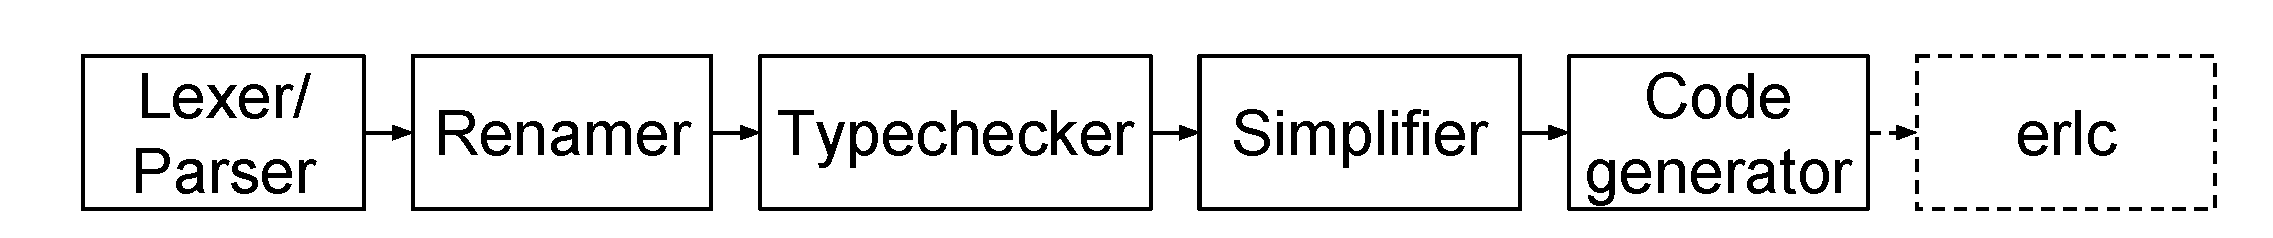
\includegraphics[width=0.6\pdfpagewidth]{figure/pipeline}}
\end{figure}

% HOW IS HOPPER BUILT

As seen in figure~\ref{fig:pipeline} the Hopper language has five steps in its 
pipeline before it turns it over to the Erlang compiler. Each step work on the 
source code representation in a uniqe way. The steps can be summerized as
follows. The lexer and parser reads in text files and converts them to an 
abstract representation, the renamer simplify this representation for that 
typechecker whos job it is to control the types of the functions. Second to last 
there is another simplifying step before the code generator which produces Core
Erlang code. The Erlang compiler is then invoked, using the produced Core Erlang
code, and the result is Erlang assembly code that is run on the BEAM VM.
